\chapter{提案}
\par
本論文では,行動情報と発話情報の両方を活用する心的状態推定システムMultimodal Inference of Mind(MIoM)を提案する.MIoMは,人間の信念や行動,発話および人間が存在する環境の状態を基に心的状態を推定する.行動情報と発話情報の両方を心的状態の推定に活用することで,発話による行動の解釈の変化や行動による発話に解釈の変化を捉え,行動情報と発話情報の相互作用を考慮して心的状態を推定する.

\par
MIoMは,環境の状態や人間の心的状態を部分的に観測可能なマルコフ決定過程(POMDP)として表される.また,心的状態とその尤度を持つパーティクルフィルタとして表され,心的状態を一意に決め付けるのではなく同時に複数保持し,時刻が経過する度に各パーティクルの尤度を更新していく.各時刻おける人間の信念や行動,発話および人間が存在する環境の状態をベイズの定理に適用し,人間が観測できていない環境領域についての信念と欲求を逐次的に推定する.


\section{関連研究との相違点}
\par
MIoMと関連研究との相違点は,行動情報と発話情報の両方を活用したマルチモーダルな心的状態推定を行う点である.MIoMは,行動情報と発話情報の両方を活用して心的状態を推定することで,発話による行動の解釈の変化や行動による発話の解釈の変化を捉え,行動情報と発話情報の相互作用を考慮した推定が可能となる.MIoMは,関連研究における問題点を解消するシステムとなっている.


\section{アルゴリズム}

\par
MIoMにおける推定処理の流れをを図\ref{fig:sys_arc}に示す.
\begin{figure}[htbp]
  \begin{center}
    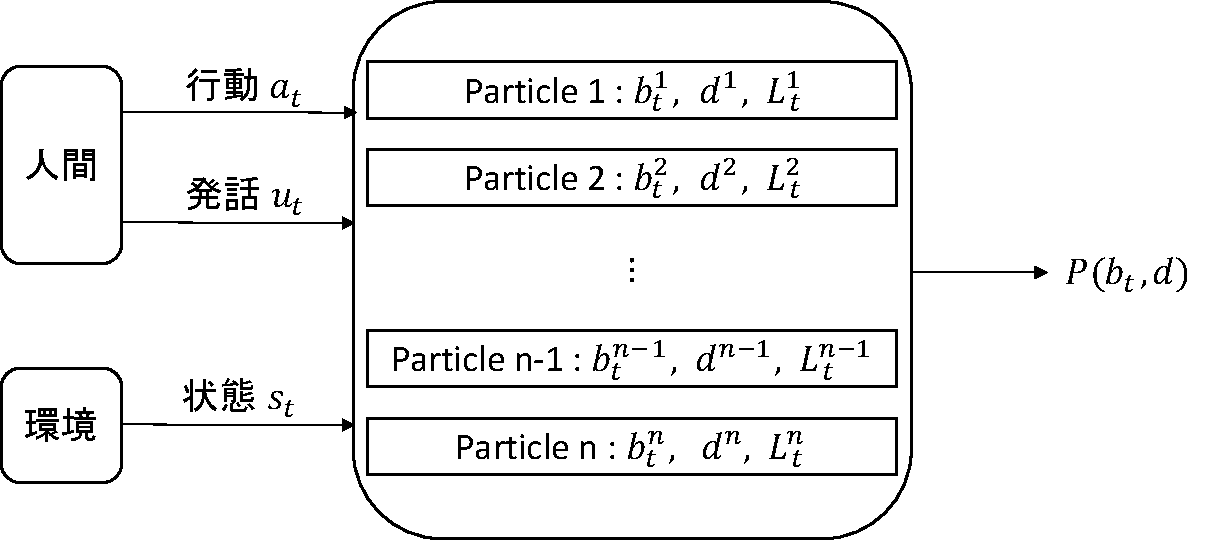
\includegraphics[scale=0.85]{./bt1.pdf}
    \caption{MIoMによる推定処理}
    \label{fig:sys_arc}
  \end{center}
\end{figure}
図\ref{fig:sys_arc}に示すように,MIoMは時刻$t$における人間の行動$a_t$,発話$u_t$および環境の状態$s_t$から信念と欲求の確率を出力する.MIoMは信念と欲求の組み合わせとその尤度を持つパーティクルフィルタとして表現され,$a_t,u_t,s_t$をベイズ推論に適用することで,それぞれのパーティクルの尤度が更新される.図\ref{fig:miom}にMIoMにおけるベイズ推論の様子を示す.
\begin{figure}[htbp]
  \begin{center}
    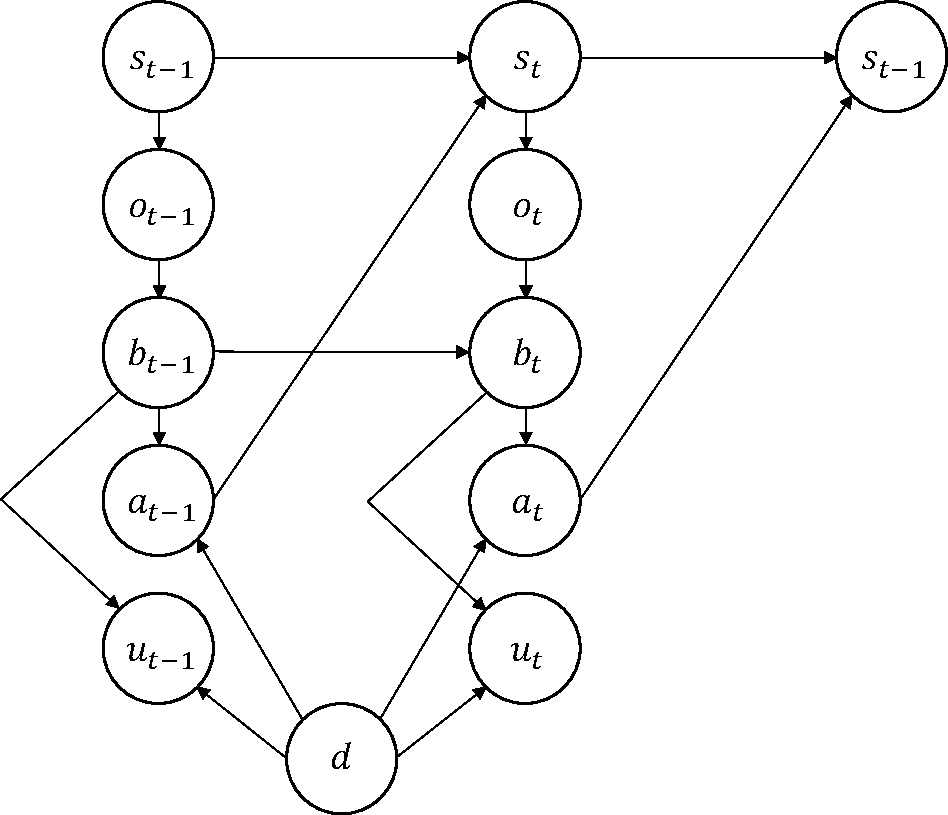
\includegraphics[scale=0.85]{./miom.pdf}
    \caption{MIoMにおけるベイズ推定}
    \label{fig:miom}
  \end{center}
\end{figure}
MIoMにおけるベイズ推論では,BToMと同様に時刻$t$における環境の状態$s_{t}$を基に人間の観測状況$o_{t}$が計算される.また,$o_{t}$を基に人間の信念$b_{t}$が計算され,$b_{t}$と人間の欲求$d$から人間の行動$a_{t}$が計算される.それに加え,$b_t$と$d$から人間の発話$u_t$が計算される.$a_{t}$および$u_t$が起こることにより,環境の状態は$s_{t+1}$に変化し,人間の観測状況,信念,行動および発話が再起的に計算される.
